\documentclass{article}
\usepackage{amsmath, amssymb, graphicx}

\title{Error Analysis of ODE Solvers: Euler vs. Runge-Kutta}
\author{Anusha Tripathi \\
Computer Science Department, Year 3 \\
St. Xavier's College (Autonomous), Kolkata}
\date{\today}

\begin{document}

\maketitle

\section{Introduction}
A differential equation is a mathematical equation that relates a function to its derivatives, describing how a quantity changes over time or space. These equations play a fundamental role in modeling natural and engineered systems, including physics, biology, economics, and engineering. Essentially, they help us understand how systems evolve over time based on given conditions.

However, most differential equations cannot be solved exactly. While there are analytical methods available for some simple cases, many real-world problems require numerical methods to approximate solutions. This is where numerical solvers such as Euler’s method and the Runge-Kutta (RK4) method come into play.

ODEs describe how a function changes with respect to an independent variable, usually time. They appear in various scientific and engineering fields, modeling phenomena like population growth, heat conduction, and motion dynamics.

In this report, we compare two widely used numerical methods: the Euler method and the fourth-order Runge-Kutta (RK4) method. We apply these methods to five different test cases: exponential decay, logistic growth, simple harmonic motion, the Lorenz system, and the Van der Pol oscillator. The goal is to evaluate their accuracy, efficiency, and convergence by comparing numerical solutions with exact analytical results where available.

\section{Mathematical Formulation}
A first-order ODE takes the general form:
\begin{equation}
    \frac{dy}{dt} = f(y, t), \quad y(0) = y_0.
\end{equation}
This equation states that the rate of change of \( y \) with respect to time \( t \) depends on the function \( f(y,t) \), with an initial value \( y_0 \) provided.

To approximate the solution, we consider the following numerical methods:

\subsection{Euler Method}
The Euler method is the simplest numerical approach to solving ODEs. It estimates the next value using a simple step-by-step approach:
\begin{equation}
    y_{n+1} = y_n + h f(y_n, t_n).
\end{equation}
This method essentially takes small steps \( h \) along the curve, using the current derivative to predict the next point. While easy to implement, Euler’s method accumulates significant errors due to its simplistic nature. The errors arise because it assumes a straight-line approximation of the curve at each step, which is not always accurate for rapidly changing functions.

\subsection{Runge-Kutta 4th Order (RK4)}
The RK4 method improves accuracy by taking weighted averages of intermediate steps. This allows it to estimate the curve more accurately within a single step. It works as follows:
\begin{align}
    k_1 &= h f(y_n, t_n) \quad \text{(Initial estimate based on the current slope)} \\
    k_2 &= h f(y_n + k_1/2, t_n + h/2) \quad \text{(Refining estimate at midpoint)} \\
    k_3 &= h f(y_n + k_2/2, t_n + h/2) \quad \text{(Further refining at midpoint)} \\
    k_4 &= h f(y_n + k_3, t_n + h) \quad \text{(Final estimate at next step)} \\
    y_{n+1} &= y_n + \frac{k_1 + 2k_2 + 2k_3 + k_4}{6}.
\end{align}
The RK4 method significantly reduces numerical errors compared to Euler’s method, making it more accurate for a given step size.

\section{Test Cases}
To compare the two methods, we analyze five different ODEs, each representing a different type of system.

\subsection{Exponential Decay}
This equation models the decay of a substance over time:
\begin{equation}
    \frac{dy}{dt} = -y, \quad y(0) = 1.
\end{equation}
The exact solution is:
\begin{equation}
    y(t) = e^{-t}.
\end{equation}
This case helps us understand how well the numerical methods approximate smooth, exponential behavior.

\subsection{Logistic Growth}
The logistic equation describes population growth under limited resources:
\begin{equation}
    \frac{dy}{dt} = y (1 - y/10), \quad y(0) = 1.
\end{equation}
Its exact solution is:
\begin{equation}
    y(t) = \frac{10}{1 + 9e^{-t}}.
\end{equation}
This test case introduces nonlinearity, making the numerical comparison more interesting.

\subsection{Simple Harmonic Motion (SHM)}
This describes oscillatory motion, such as a mass on a spring:
\begin{equation}
    \frac{dx}{dt} = v, \quad \frac{dv}{dt} = -\omega^2 x.
\end{equation}
The exact solution is:
\begin{equation}
    x(t) = A \cos(\omega t) + B \sin(\omega t).
\end{equation}
This test demonstrates how well numerical methods handle periodic motion.

\subsection{Lorenz System (Chaotic Behavior)}
This set of equations models chaotic fluid flow:
\begin{align}
    \frac{dx}{dt} &= \sigma (y - x), \\
    \frac{dy}{dt} &= x(\rho - z) - y, \\
    \frac{dz}{dt} &= xy - \beta z.
\end{align}
Small numerical errors grow rapidly in chaotic systems, making this a challenging test case.

\subsection{Van der Pol Oscillator}
This equation models nonlinear oscillations:
\begin{equation}
    \frac{d^2x}{dt^2} - \mu(1 - x^2) \frac{dx}{dt} + x = 0.
\end{equation}
Rewriting it as a system:
\begin{align}
    \frac{dx}{dt} &= v, \\
    \frac{dv}{dt} &= \mu(1 - x^2)v - x.
\end{align}
This test helps evaluate how numerical solvers handle nonlinear damping effects.

\section{Error Analysis}
To measure numerical errors, we compute the L2 norm of the error:
\begin{equation}
    E = \frac{\| y_{\text{exact}} - y_{\text{numerical}} \|_2}{N}.
\end{equation}
The observed errors for each method are summarized in Table \ref{tab:errors}.

\begin{table}[h]
    \centering
    \begin{tabular}{|l|c|c|c|} \hline
    Method & L2 Error & Max Error & RMSE \\ \hline
    Euler (Exponential Decay) & 0.000570 & 0.009489 & 0.005696 \\ \hline
    RK4 (Exponential Decay) & 0.000000 & 0.000000 & 0.000000 \\ \hline
    Euler (Logistic Growth) & 0.003789 & 0.064599 & 0.037889 \\ \hline
    RK4 (Logistic Growth) & 0.000000 & 0.000000 & 0.000000 \\ \hline
    Euler (SHM) & 0.008573 & 0.269985 & 0.121248 \\ \hline
    RK4 (SHM) & 0.000000 & 0.000000 & 0.000000 \\ \hline
    Euler (Lorenz) & 0.087143 & 6.420071 & 2.755716 \\ \hline
    Euler (Van der Pol) & 0.020209 & 0.812551 & 0.285801 \\ \hline
    \end{tabular}
    \caption{Numerical Errors for Different Methods}
    \label{tab:errors}
\end{table}


\clearpage
\section{Results and Visualizations}
We provide graphical comparisons for each test case to illustrate the accuracy of the numerical methods- Euler and RK4. The exact solutions for the first three equations have also been plotted. It is clear that RK4 is much more accurate, and in the case of SHM, the accuracy of the methods compared to the exact solution is very apparent.
\begin{center}
    \begin{figure}[htbp]
        \centering
        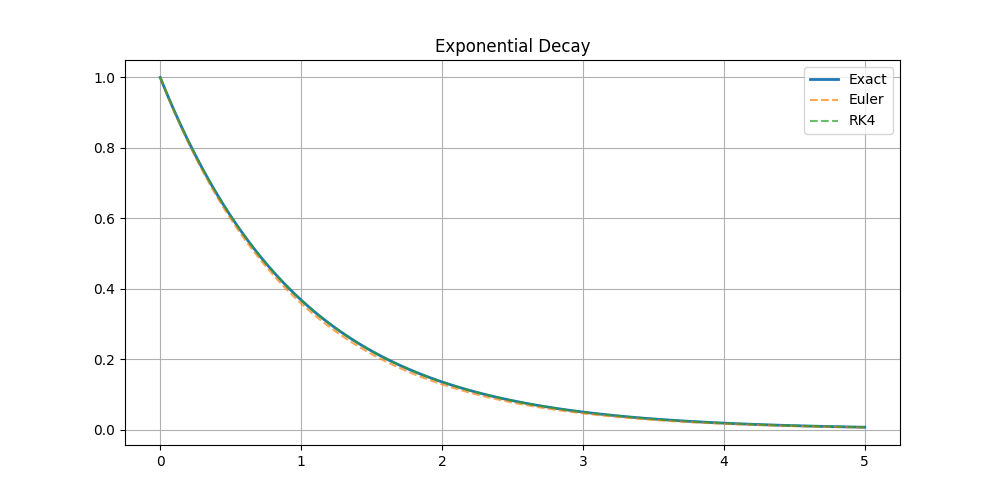
\includegraphics[width=0.7\textwidth]{results/figures/exponential_decay.png}
        \caption{Numerical vs Exact Solution for Exponential Decay.}
        \label{fig:exp_decay}
    \end{figure}
    
    \begin{figure}[htbp]
        \centering
        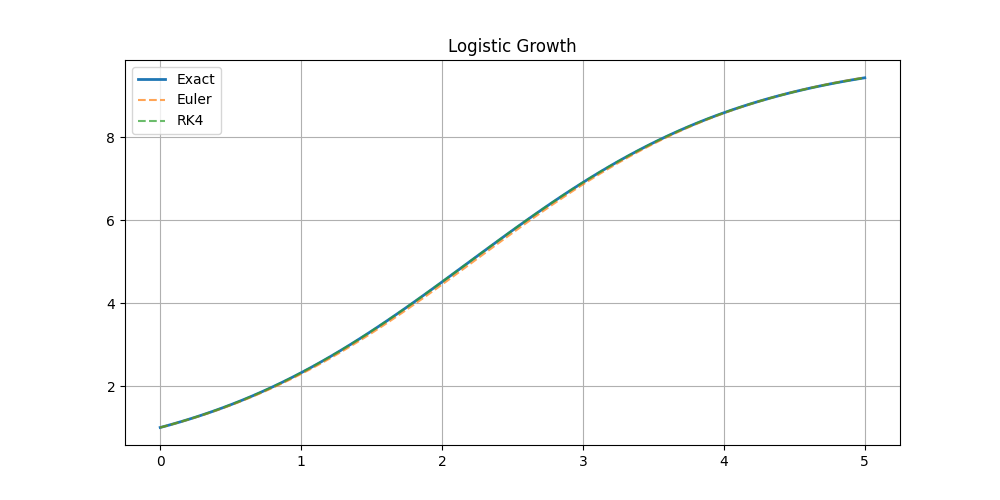
\includegraphics[width=0.7\textwidth]{results/figures/logistic_growth.png}
        \caption{Numerical vs Exact Solutions for Logistic Growth.}
        \label{fig:logistic_growth}
    \end{figure}
    
    \begin{figure}[htbp]
        \centering
        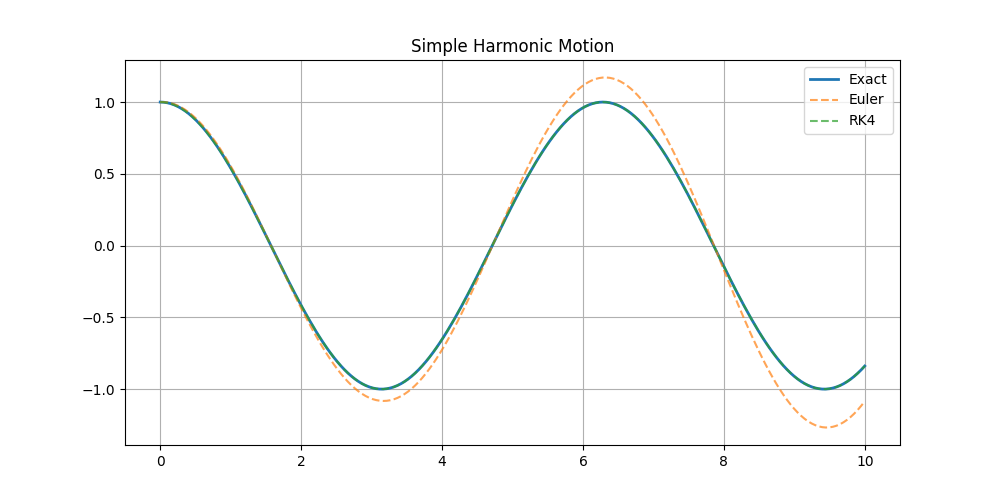
\includegraphics[width=0.7\textwidth]{results/figures/shm.png}
        \caption{Numerical vs Exact Solutions for Simple Harmonic Motion.}
        \label{fig:shm}
    \end{figure}
    
    \begin{figure}[htbp]
        \centering
        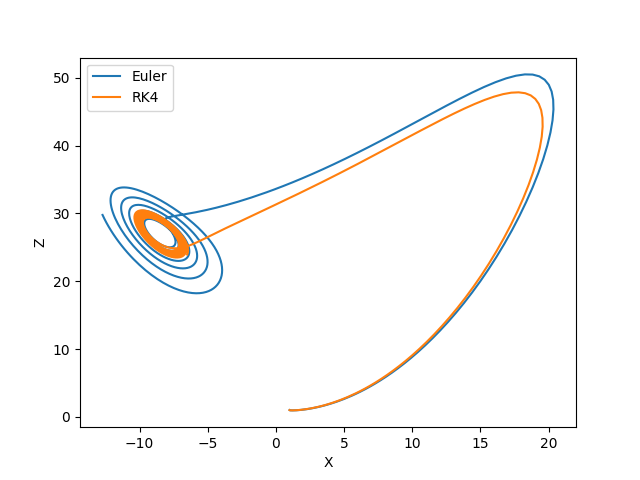
\includegraphics[width=0.7\textwidth]{results/figures/lorenz.png}
        \caption{Euler vs RK4 Solutions for the Lorenz System.}
        \label{fig:lorenz}
    \end{figure}
    
    \begin{figure}[htbp]
        \centering
        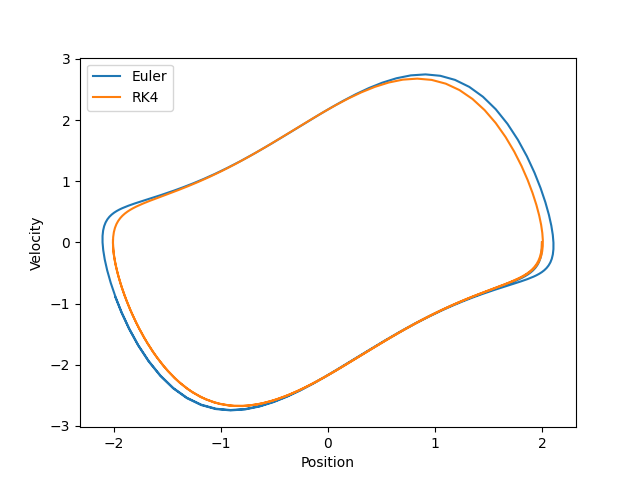
\includegraphics[width=0.7\textwidth]{results/figures/vdp.png}
        \caption{Euler vs RK4 Solutions for the Van der Pol Oscillator.}
        \label{fig:vanderpol}
    \end{figure}
    \end{center}
    
    \clearpage  % Ensures figures appear before the Conclusion
    
\section{Conclusion}
Our analysis shows that RK4 significantly outperforms the Euler method in terms of accuracy. The Euler method introduces large errors, making it less suitable for precise computations. The Van der Pol oscillator further highlights Euler’s instability in nonlinear cases. RK4 achieves much smaller errors and better convergence properties, making it the preferred choice for solving ODEs numerically.

Next steps include comparing more complex differential equations with their exact solutions and exploring the use of PETSc modules to analyze error differences. Additionally, future work could explore adaptive step-size techniques to optimize the trade-off between accuracy and computational efficiency. Another promising direction is incorporating Verlet integration, particularly for second-order systems like harmonic motion and chaotic dynamics, where it provides better energy conservation and stability over long time steps.

\end{document}

